\levelB{Exploratory research of models based on accuracy}
\label{sec:evalmodels}

\levelC{Objective}
In this exploratory research, different neural networks are trained and validated
at the file fragment identification task. Their accuracy is then compared,
to identify which models should be considered or disregarded in the remaining phases.


\levelC{Sampling}
To select a sample instance from the Govdocs1 dataset, first a random file is selected among those available, without replacement. Then, a block from this file is randomly selected. After all files have participated in the process, the process may be repeated as long as necessary. This way, all files are considered and the classes are easily balanced.
This contrasts with the sampling technique applied in other works, where all the sectors are grouped before sampling, which may lead to an imbalance between classes.

\levelC{Inputs}
%one-hot
The input features of the network for each instance is a 512x256 matrix representing only one block of 512 bytes of a random file of the dataset. Each of the 512 bytes is one-hot encoded, meaning that its value is converted into a vector with 256 elements, with only one of them set to 1, corresponding to the value of the byte, while the others are set to zero. A batch size of 100 was used, with 28 steps per epoch.

%8bits
% The input features of the network for each instance is a 512x8 matrix representing only one block of 512 bytes of a random file of the dataset. Each of the 512 bytes uses a custom encoding where each of the 8 bits of a byte is represented as -1 or 1, depending whether the bit is 0 or 1. During initial tests, this encoding was compared to three other encodings: one-hot encoding, 8 bits represented as 0 or 1\todo{include citation}, and 8 bits represented as [0,1] and [1,0] \cite{hiester_file_2018}. More research should be done in the future to determine the best of the four, but initial results suggest they have similar impact on the model accuracy. The one-hot encoding has the disadvantage of increasing the input matrix size by a factor of 32.

\levelC{Outputs}
The output of the network for a given instance is a vector with a size equal to the number of classes, subjected to a softmax function, which applies the exponential function on the vector and then normalizes it. Each value will represent the predicted probability that the instance belongs to a specific class.


\levelC{Models}
The networks under consideration used different combinations of convolutional, max pooling, LSTM, and fully connected layers,
%loss
applying categorical cross-entropy as the loss function. Binary cross-entropy and mean squared error were considered during initial tests, but categorical cross-entropy gave faster training times.

Fourteen models participated in this evaluation. One of then is a simple single-layer perceptron. Two of them use LSTM layers without convolutional layers, while 3 of them use convolutional layers without LSTM layers. Eight models combine convolutional layers and LSTM layers. Table \ref{tab:models} outline the parameters of the models, which can be analyzed in more detail in the code repository \sloppy\url{http://github.com/atilaromero/randomness-experiments}. The convolutional layers do not use padding. 

\newcommand{\paint}{\cellcolor{gray!25}}
\begin{table}[!ht]
    \centering
    \footnotesize
    \caption{14 models trained on 30 classes}
    \label{tab:models}
\begin{tabular}{l||l|l|l||l|l|l||l|l||l}
\hline
Model  & \multicolumn{3}{l||}{Convolutional layers} & \multicolumn{3}{l||}{Max pooling} & \multicolumn{2}{l||}{LSTM} & Dense  \\ \hline
       & output       & window       & stride      & pool    & stride    & channel    & output     & return       & output \\ 
       & size         & size         & length      & size    & length    & first      & size       & sequences    & size   \\ \hline
                                                                                                                              \hline
D      & \paint       & \paint       &     \paint  & \paint  &  \paint   & \paint     & \paint     & \paint       & 30     \\ \hline
LD     & \paint       & \paint       &     \paint  & \paint  &  \paint   & \paint     & 32         & no           & 30     \\ \hline
LL     & \paint       & \paint       &     \paint  & \paint  &  \paint   & \paint     & 32         & yes          & \paint \\ 
       & \paint       & \paint       &     \paint  & \paint  &  \paint   & \paint     & 32         & no           & \paint \\ \hline
CD     & 64           & 64           & 8           & \paint  &  \paint   & \paint     & \paint     & \paint       & 30     \\ \hline
CM     & 30           & 32           & 1           & 481     & 1         & no         &  \paint    & \paint       & \paint \\ \hline
CCM    & 30           & 32           & 1           &         &           &            & \paint     & \paint       & \paint \\ 
       & 30           & 2            & 2           & 240     & 1         & no         & \paint     & \paint       & \paint \\ \hline
CL     & 30           & 32           & 32          & \paint  &  \paint   & \paint     & 30         & no           & \paint \\ \hline
CML    & 32           & 32           & 32          & 2       & 2         & yes        & 30         & no           & \paint \\ \hline
CLL    & 32           & 32           & 32          & \paint  &  \paint   & \paint     & 64         & yes          & \paint \\ 
       &              &              &             & \paint  &  \paint   & \paint     & 30         & no           & \paint \\ \hline
CLD    & 256          & 16           & 16          & \paint  &  \paint   & \paint     & 128        & no           & 30     \\ \hline
CCL    & 128          & 8            & 8           & \paint  &  \paint   & \paint     &            &              & \paint \\ 
       & 64           & 8            & 8           & \paint  &  \paint   & \paint     & 30         & no           & \paint \\ \hline
CCLL   & 128          & 8            & 8           & \paint  &  \paint   & \paint     & 64         & yes          & \paint \\ 
       & 64           & 8            & 8           & \paint  &  \paint   & \paint     & 30         & no           & \paint \\ \hline
CMCML  & 128          & 8            & 8           & 2       & 2         & yes        &            &              & \paint \\ 
       & 64           & 8            & 8           & 2       & 2         & yes        & 30         & no           & \paint \\ \hline
CMCMLL & 128          & 8            & 8           & 2       & 2         & yes        & 64         & yes          & \paint \\ 
       & 64           & 8            & 8           & 2       & 2         & yes        & 30         & no           & \paint \\ \hline
\end{tabular}
\end{table}

%optimization
All the trainings used the Adam \cite{kingma_adam:_2014}
optimization algorithm to guide backpropagation, which was selected because it performed well in the preliminary results without fine-tuning of parameters.

% Constraints
The models were trained until no further improvement was observed in the last 10 epochs.

\levelC{Results}
%exp18
The two models that used LSTM layers without convolutional layers presented slower learning in comparison with the others, as can be seen in figure \ref{fig:learning}. The validation accuracy values can be consulted in figure \ref{fig:models}.

\noindent
\begin{figure*}[htb!]
\centering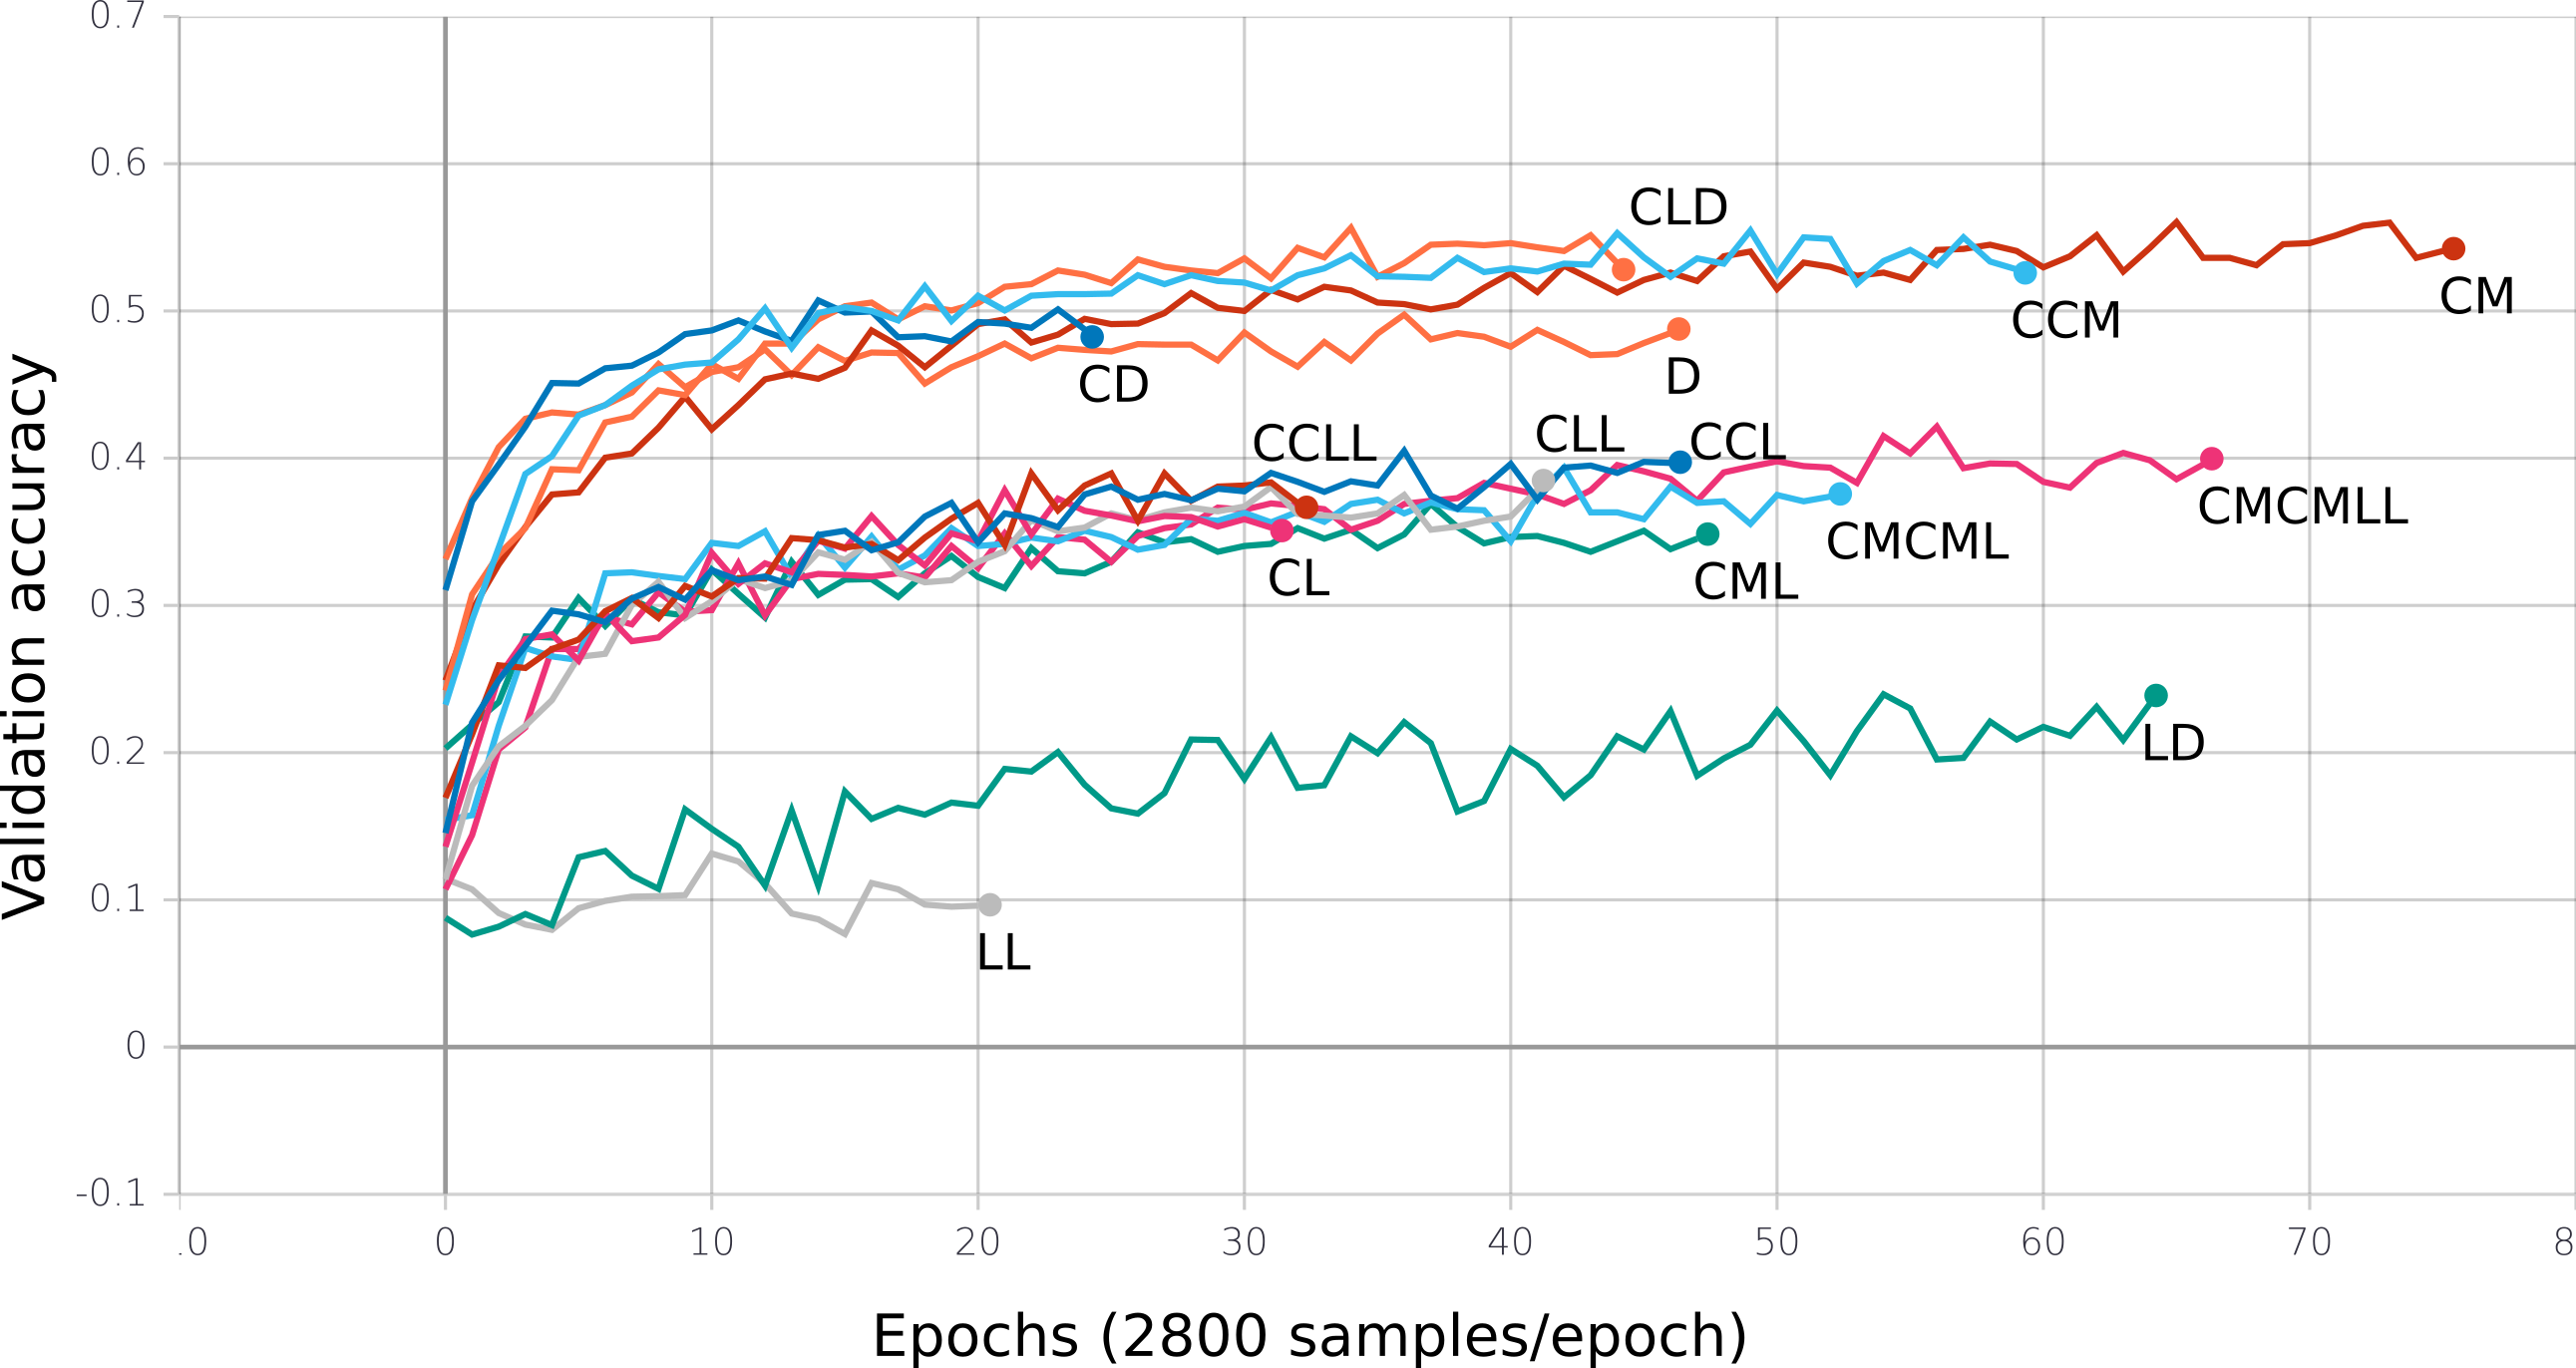
\includegraphics[width=0.9\textwidth]{content/epoch_val_categorical_accuracy.png}
\caption{\label{fig:learning}Learning curves of some models (validation accuracy vs. time)}%
\end{figure*}

\noindent
\begin{figure*}[htb!]
\centering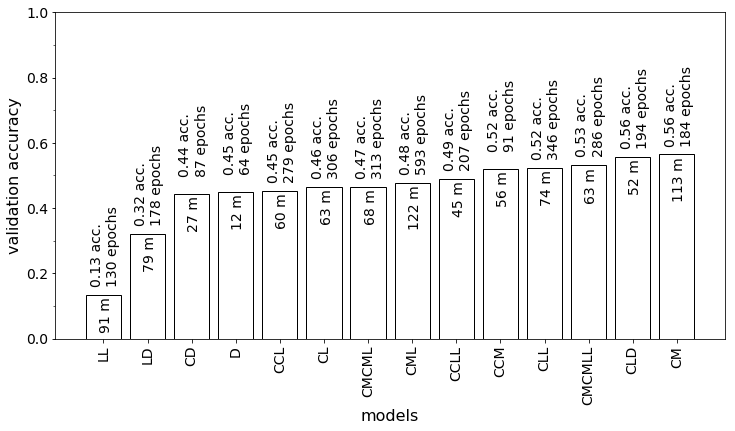
\includegraphics[width=1.0\textwidth]{content/models.png}
\caption{\label{fig:models}The bar plot shows the validation accuracy of the considered models. Their training time, in minutes, and the total epochs processed is also indicated. The training was interrupted when no further improvement was observed for 10 consecutive epochs.}%
\end{figure*}


The validation accuracy values of the remaining models were in the 0.35-0.54 range.

The selected model for further research, identified as ``CM'', achieved an accuracy of 0.54. The models, ``CLD'' and ``CCM'' achieved similar values, but model ``CM'' performed better in the experiment described in section \ref{sec:exprandom}.

To check if the two slower models could give better results if executed for a longer period, they were trained for 10 hours. The model identified as ``LD'', which uses an LSTM layer followed by a fully connected layer, was able to achieve an accuracy of 0.494, while the other, ``LL'', achieved only 0.153.

%stagnation in learning with such short times, combined with low final accuracy suggests that the dataset present some patterns that are easily recognizable, while the rest of the dataset present a very hard classification task.

% \levelC{Limitations and threats to validity}
In this exploratory research, the models were not trained until exhaustion. This was initially done to identify which models would be most promising for future testing, but further attempts to tune layer types, quantity and parameters resulted in accuracy values still close to 0.54, which suggests that selection or tuning of models may not be the best approach to improve results.
